\begin{figure}[htbp]
  \centering
  \caption{Confronto frente à Melhor Solução Conhecida (BKS) nas instâncias \texttt{B/0012} ($\lvert\mathcal{A}'\rvert = 11$ corredores) e \texttt{B/0013} ($\lvert\mathcal{A}'\rvert = 9$ corredores). Com o número ótimo de corredores fixado, o refinamento em nível de pedidos do \texttt{GVNS} empacota até $+8$ unidades extras em \texttt{B/0012} ($f^* = 568{,}36$) e $+1$ unidade em 100\% das sementes em \texttt{B/0013} ($f^* = 757{,}11$), enquanto \texttt{Santos e Baldotto (2025)} estaciona em $-2$ unidades abaixo do BKS em \texttt{B/0013}.}
  \label{fig:novas_msc_comparativo}
  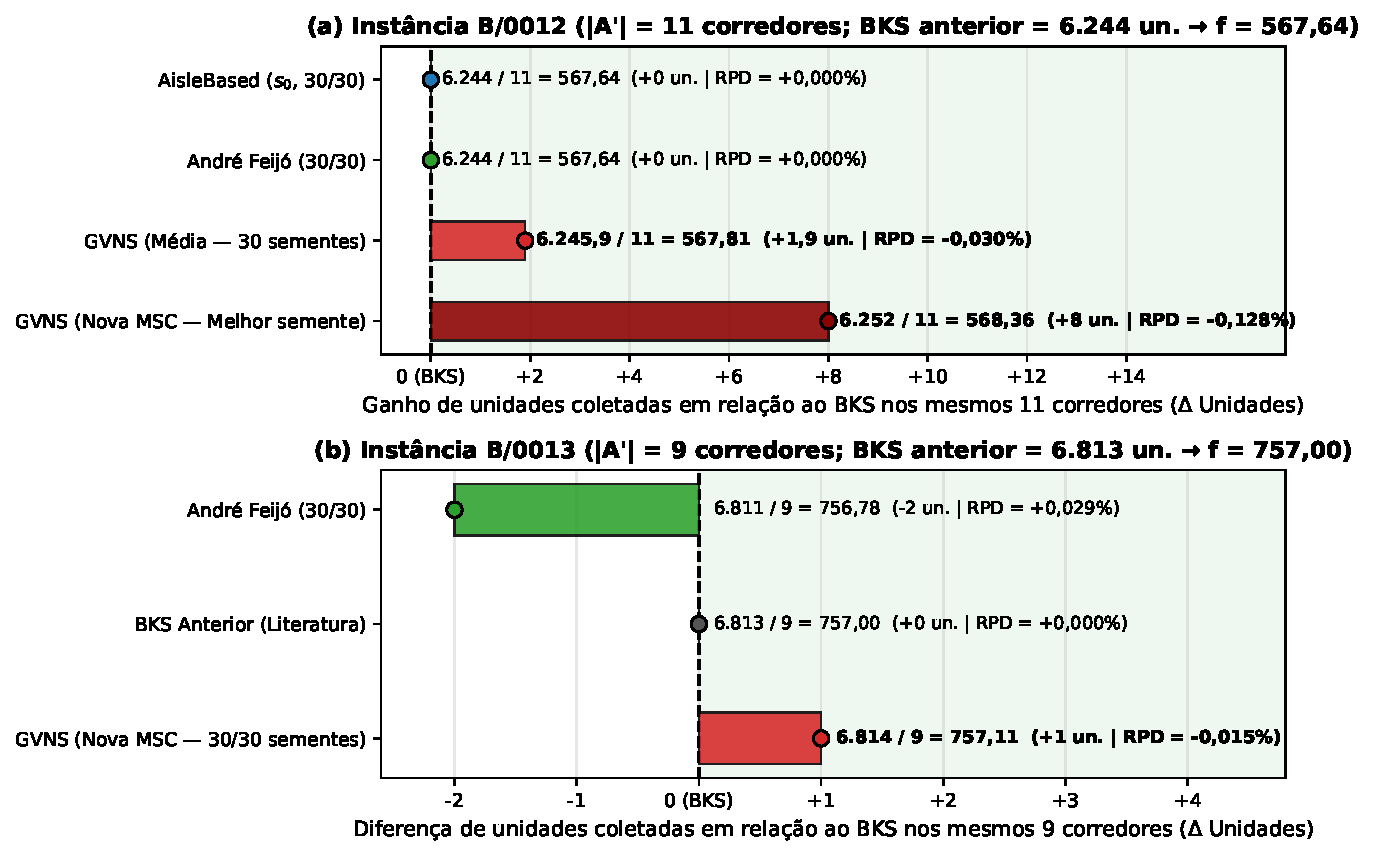
\includegraphics[width=0.9\textwidth]{img/novas_msc_comparativo.pdf}
  \caption*{\footnotesize Fonte: Elaborado pelo autor, 2026.}
\end{figure}
